\chapter{Elliptic curve cryptography}
\label{chpr:ecc}
In this chapter we will analyse the cryptographic primitives and assumptions that will allow in the next chapter to introduce the digital signature schemes that are the core of the present work. The first argument will be the specialization of elliptic curves to finite fields, the mathematical structure underpinning the whole elliptic curve cryptography.

\bigskip

\section{Elliptic curves over finite fields}
\label{ecoverff}
Up to now we considered the field over which the curve is defined to be the set of real numbers: this is not at all the unique possibility. The typical choice in cryptography is $K = \mathbb{F}_p$, where $\mathbb{F}_p$ is the finite field with $p$ elements. 
\\
Since there are only finitely many pairs $(x, y)$ with $x, y \in \mathbb{F}_p$, the group $E(\mathbb{F}_p)$ is finite.
In practice we consider: 
$$\{(x, y) \in \mathbb{F}_p^2 \ | \ y^2 \equiv x^3 + ax + b \ (\text{mod} \ p), \ 4a^3 + 27b^2 \not\equiv 0 \ (\text{mod} \ p)\} \cup \{\infty\}.$$
It can be shown that the formulas for point addition are the same derived in Section \ref{grouplaw}, but where the calculations are done modulo $p$\footnote{Notice that reduction modulo $p$ can be executed much faster if the prime $p$ is a Mersenne or a pseudo-Mersenne prime, i.e. if $p = 2^d - 1$ for some $d$ in the first case or if $p \simeq 2^d$ in the second one.}.
\\
\begin{center}
	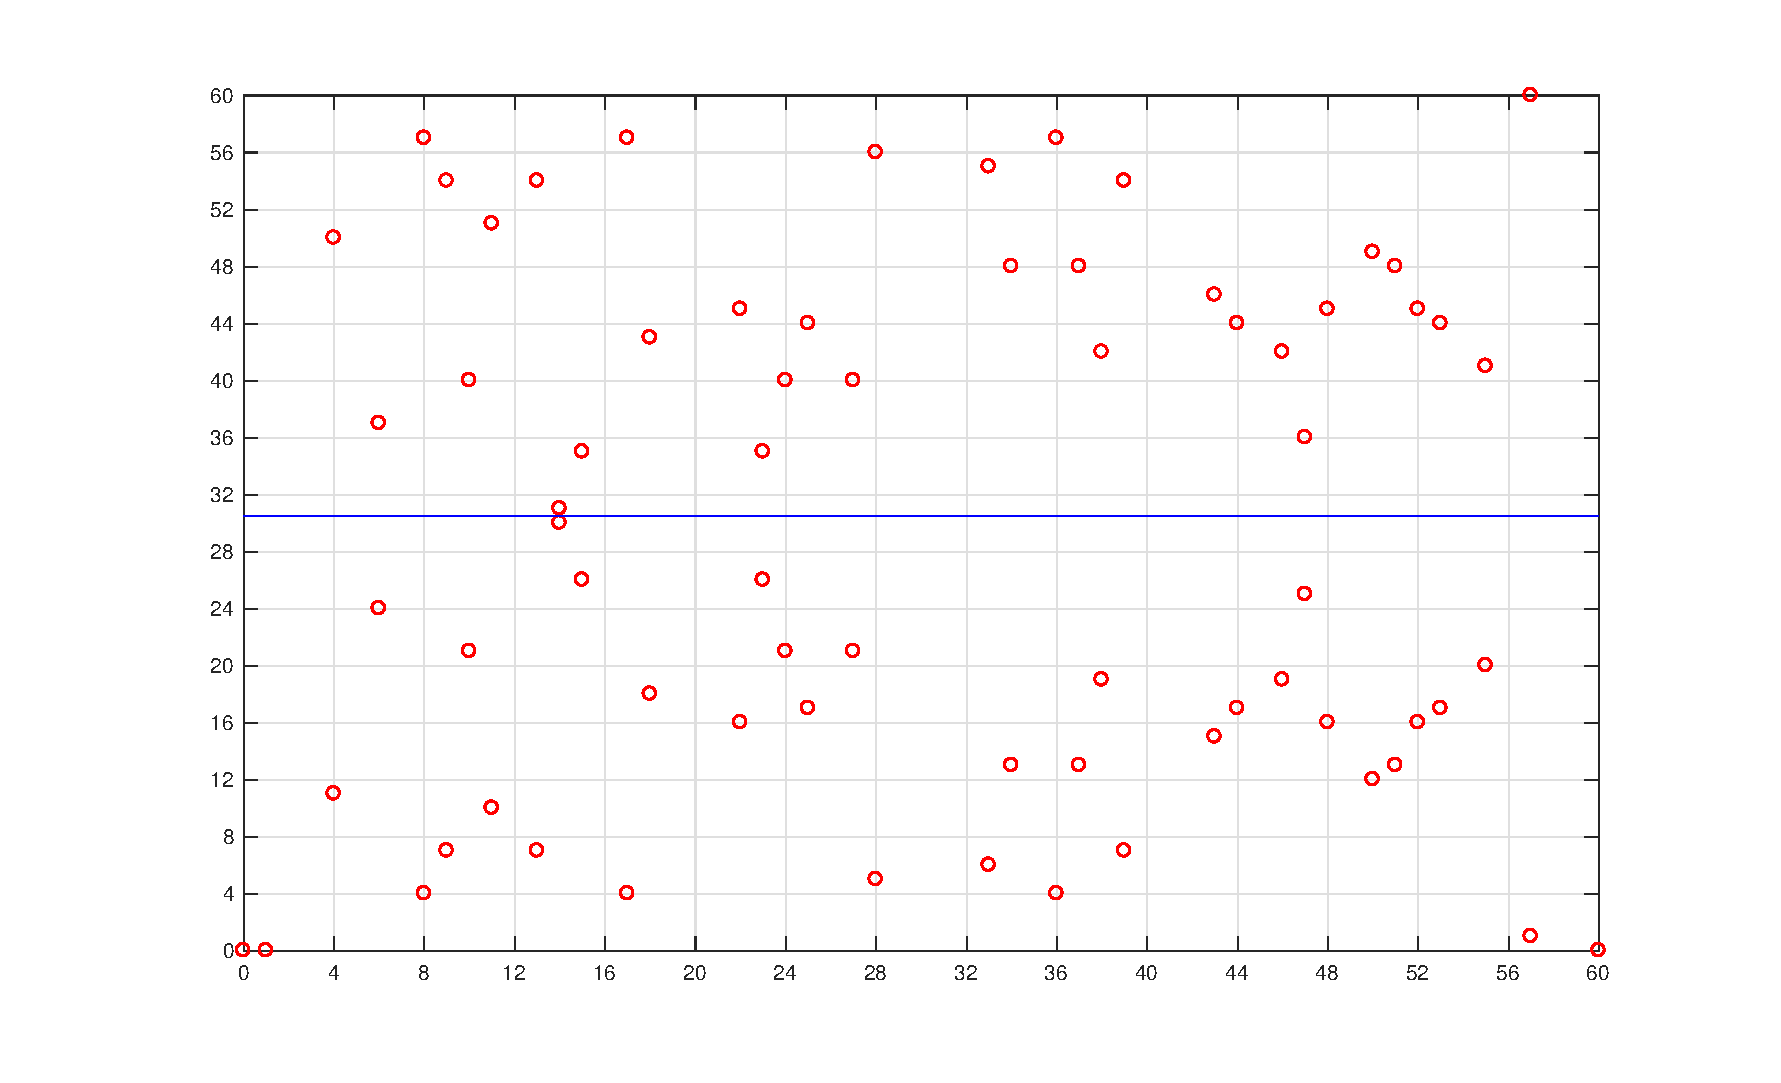
\includegraphics[width=0.9\linewidth]{Images/ec_over_ff.eps}
	\captionof{figure}{The curve $y^2 = x^3 - x$ over $\mathbb{F}_{61}$.}
	\label{fig:figure4}
	\source{\url{https://en.wikipedia.org/wiki/Elliptic_curve\#Elliptic_curves_over_finite_fields}.}
\end{center}
In Figure \ref{fig:figure4} it is represented the typical shape of an elliptic curve over a finite field: we can see that we are not anymore dealing with a smooth curve, but with a finite set of points scattered along the plane. We can notice a certain degree of symmetry with respect to the line $y = \frac{p}{2}$, with the exception of the points with $y$ coordinate equal to zero, that correspond to the roots of the cubic $x^3 + ax + b$ in $\mathbb{F}_p$.
\\
It is still possible to define a geometric method for point addition: the general idea is that we draw the line passing through the points considered. Since we are working in modular arithmetic, this line "repeats" itself along the plane. Once the line intersects a third point, we take the opposite one to be the result of the addition. The approach is presented in Figure \ref{fig:figure5}, however the method can be somewhat counterintuitive, especially when dealing with point doubling, so we stick with the algebraic notation.

\bigskip
\noindent
The number of points on an EC over $\mathbb{F}_q$ plays a central role in the cryptographic applications, so we state here a useful theorem that allows to give an estimate:
\begin{thm} [{\bf Hasse's theorem}] Let $\mathbb{F}_q$ be a finite field and let $E$ be an elliptic curve defined over $\mathbb{F}_q$. Then the order of $E(\mathbb{F}_q)$ (i.e. the number of points) satisfies: $$|q + 1 - \#E(\mathbb{F}_q)| \leq 2\sqrt{q}$$
\end{thm}
\begin{center}
	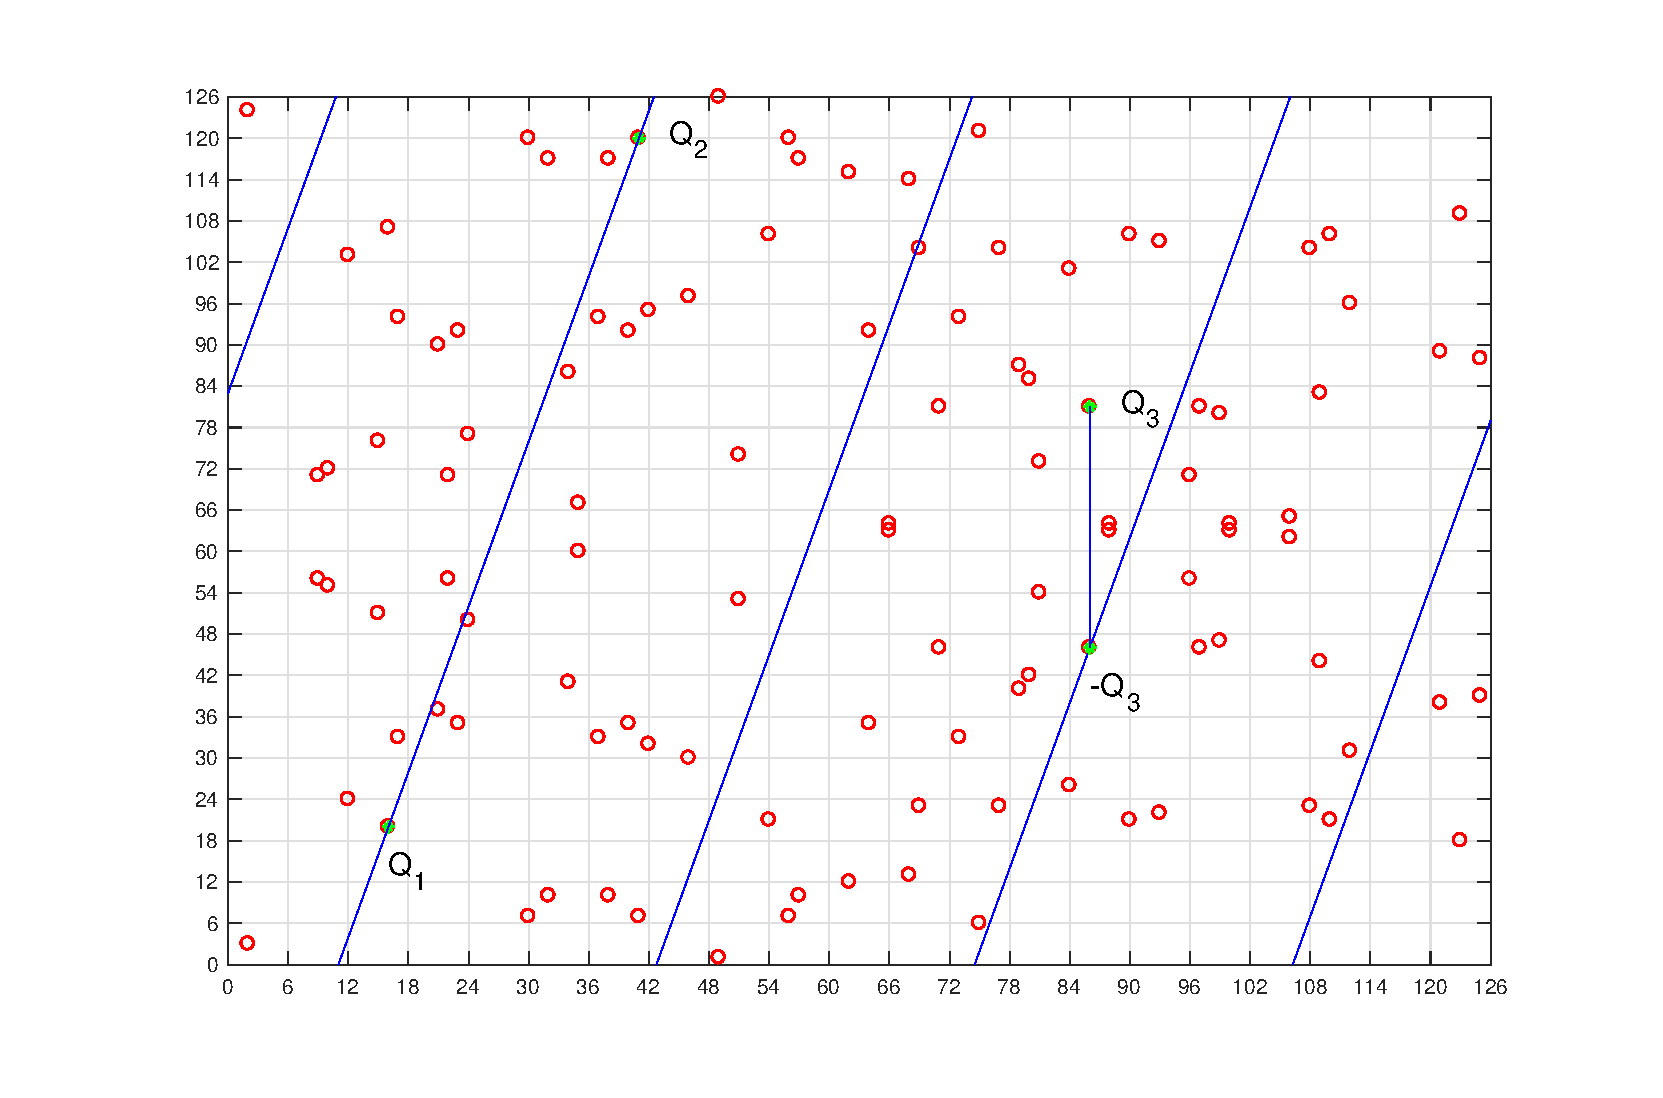
\includegraphics[width=0.9\linewidth]{Images/sum_ec_over_ff.eps}
	\captionof{figure}{Geometric representation for the addition of points on the elliptic curve $y^2 = x^3 - x + 3$ over $\mathbb{F}_{127}$.}
	\label{fig:figure5}
	\source{\cite{RefWork:4}.}
\end{center}
\noindent
Loosely speaking, Hasse's theorem tells us that the number of points over $E(\mathbb{F}_q)$ increases linearly with the order of the field.
\\
Another observation we want to do is that if $\#E(\mathbb{F}_p)$ is a prime number, then $E(\mathbb{F}_p)$ is a cyclic group: this is a direct consequence of Lagrange's theorem. Since the order of each subgroup is a divisor of the order of the group, we have that, if the order of the group is a prime number, there is no subgroup (with the exception of the trivial one, comprising only the point at infinity). This means that it has to exist a generator of the whole group. Suppose this is not the case, i.e. $\nexists G \in E(\mathbb{F}_p) \ | \ \forall Q \in E(\mathbb{F}_p) \ \exists q \in [1, ..., \#E(\mathbb{F}_p)] \ \text{s.t.} \ Q = qG$: thus, $\forall G \in E(\mathbb{F}_p)$, there exists at least a $Q$ for which the relation $Q = qG$ does not hold. Fix $G$ and start adding it repeatedly to itself. Of course we would reach different points in $E(\mathbb{F}_p)$ due to the closure of the addition. However we won't be able to reach $Q$, by definition. But eventually we would reach the point at infinity (when $q$ gets equal to the order of $G$): then we would start again, meaning that we would have found a cyclic subgroup. But this is in contrast with Lagrange's theorem, so that we can conclude that the whole set of elliptic curve's points form a cyclic group if $\#E(\mathbb{F}_q)$ is a prime number.

\bigskip

\subsection{Elliptic curve domain parameters}
\label{ecparam}
In order to rely on ECC, the parties involved in a scheme need to agree on a set of parameters called elliptic curve domain parameters. A typical choice is to rely on standardized curves (e.g. those defined in \cite{RefWork:3}); however, it is still possible to choose other parameters, but this has to be done carefully, as we will explain in this section. We start defining EC parameters, following closely \cite{RefWork:2}.
\\
\\
Elliptic curve parameters are defined as a sextuple $T = (p, a, b, G, n, h)$, where:
\begin{itemize}
	\item The integer $p$ specifies the prime finite field $\mathbb{F}_p$;
	\item The two elements $a, b \in \mathbb{F}_p$ specifies the elliptic curve $E(\mathbb{F}_p)$ through the Weierstrass equation;
	\item $G$ is a point on $E(\mathbb{F}_p)$;
	\item $n$ is the order of $G$, i.e. the number of elements of the cyclic subgroup generated by $G$ (that can coincide with the whole $E(\mathbb{F}_p)$);
	\item $h = \frac{\#E(\mathbb{F}_p)}{n}$ is an integer\footnote{We can deduce that $h$ is an integer directly from Lagrange's theorem.} called the cofactor. 
\end{itemize}
There are different ways in which we can choose these parameters. For example, they can be generated at random or not. Random generation is a conservative choice, since it offers a guarantee against future special purpose attacks. In this case it could be better to use verifiable random parameters, meaning that $(a, b)$ and/or $G$ are obtained as output from a secure hash function\footnote{An hash function in general is a function that takes as input strings of arbitrary length and outputs in a fixed length sequence of bytes. For a discussion on the security properties of an hash function we refer to the appendix of \cite{RefWork:2}.}, applied to some seed $S$. When choosing verifiable random parameters, the sextuple $T$ should be coupled with the seed value $S$ to allow parameters' validation. However, non random curves are typically built in particular ways to ensure efficient computations. Standardized curves, that comprises both types of EC, have the advantage of underpinning interoperability, plus an high degree of reliability, having been heavily tested.
\\
Now that we have explained what they are and how they can be chosen, we will show some constraints and the validation process for the sextuple $T$.

\bigskip
\bigskip
\bigskip
\bigskip
\bigskip
\noindent
{\bf Parameters' selection}: 
\begin{enumerate}
	\item Select the approximate security level in bits, $t$\footnote{The security level should be chosen such that solving the ECDLP requires $2^t$ curve's operations. The SEC standard that we are following restricts to $t \in \{80, 112, 128, 192, 256\}$.};
	\item Choose a prime $p$ such that $\lceil log_2p\rceil = 2t$ if $80 < t < 256$, such that $\lceil log_2p\rceil = 521$ if $t = 256$ and such that $\lceil log_2p\rceil = 192$ if $t = 80$;
	\item Select $a$ and $b$ in $\mathbb{F}_p$ such that:
	\begin{itemize}
		\item $4a^3 + 27b^2 \neq 0 \ (\text{mod} \ p)$;
		\item $\#E(\mathbb{F}_p) \neq p$;
	\end{itemize} 
	\item Select $G \in E(\mathbb{F}_p)$ such that:
	\begin{itemize}
		\item $p^B \neq 1 \ (\text{mod} \ n), \ \forall 1 \leq B < 100$;
		\item $h \leq 2^{\frac{t}{8}}$;
		\item $n - 1$ and $n + 1$ should each have a large prime factor $r$, which is large in the sense that $log_nr > \frac{19}{20}$.
	\end{itemize}
\end{enumerate}
These requirements may look strange, but are all needed in order to avoid special attacks. In particular, the two requirements at point 3 are needed in order for the curve to be non singular and to avoid Smart's attack\footnote{The points on the curve are mapped to the elements of the additive group of $\mathbb{F}_p$, so that the discrete logarithm problem is solvable in polynomial time through the {\bf Extended Euclidean Algorithm}.}, respectively.
\\
The three requirements at point 4 instead are needed to ensure that the curve is robust against MOV and Cheon's attack\footnote{These attacks are complex and their explanation is out of the scope of the present work; we refer the interested reader to the appendix of \cite{RefWork:2} for an overview and for further bibliography.}, and to ensure that the order of $G$ is sufficiently high.
\\
Notice however that the choice of the parameters does not secure against all possible attacks. Indeed other kind of attacks may be possible, such as side channel attacks: timing and power analysis are an example. They exploit the differences in the point addition and doubling operations, that lead to different timings or power consumptions. Possible solutions are a change of coordinates or the use of Edwards curves, a special family of elliptic curves for which addition and doubling can be done with the same operation.

\bigskip
\noindent
{\bf Parameters' validation}: Given $T = (p, a, b, G, n, h)$ and $t$, the parameters are deemed valid if:
\begin{enumerate}
	\item $p$ is a prime such that $\lceil log_2p\rceil = 2t$ if $80 < t < 256$, or such that $\lceil log_2p\rceil = 521$ if $t = 256$, or such that $\lceil log_2p\rceil = 192$ if $t = 80$;
	\item $a, b, x_G$ and $y_G$ are integers in $[0, ..., p - 1]$;
	\item $4a^3 + 27b^2 \neq 0 \ (\text{mod} \ p)$;
	\item $y_G^2 = x_G^3 + ax_G + b \ (\text{mod} \ p)$;
	\item $n$ is a prime number;
	\item $h \leq 2^{\frac{t}{8}}$ and $h = \lfloor (\sqrt{p} + 1)^2 / n \rfloor$;
	\item $nG = \infty$;
	\item $p^B \neq 1 \ (\text{mod} \ n), \ \forall 1 \leq B < 100$ and $n \neq p$. 
\end{enumerate}
If the parameters are verifiably random, it should also be checked that $(a, b)$ and/or $G$ have been correctly derived from the seed $S$.
\\
These checks are needed to verify that: the curve has the required difficulty level, it is defined over $\mathbb{F}_p$, it is non singular, $G$ is a point of the curve, the DL is difficult, $h$ is effectively the cofactor of $G$, $G$ has order $n$ and neither MOV nor Smart's attacks are possible.

\bigskip

\subsection{Elliptic curve key pairs}
\label{keypairs}
In this section we would like to briefly analyse the core of the public key cryptography based on elliptic curves: the concept of elliptic curve key pair. Shortly, public key cryptography is a cryptographic system that relies on pairs of keys, a public and a private key, with different roles. The asymmetry of the keys is the reason behind the fact that public key cryptography is sometimes called also asymmetric cryptography. We talk about asymmetry since public keys can be published, while private keys must be kept secret, as the names suggest. This accomplishes two functions: authentication, since everybody with the public key can verify that the holder of the paired private key sent a signed message, and encryption, where the public key is used for encryption, but only the owner of the private counterpart can decrypt.

\bigskip
\noindent
Given some elliptic curve domain parameters $T = (p, a, b, G, n, h)$, an elliptic curve key pair $\{\textcolor{red}{q}, \textcolor{green}{Q}\}$ associated with $T$ consists of an elliptic curve secret key $\textcolor{red}{q}$, which is an integer in $[1, n - 1]$, and an elliptic curve public key $\textcolor{green}{Q} = (x_Q, y_Q)$, which is the point $\textcolor{green}{Q} = \textcolor{red}{q}G$.
\\
The choice of the colours is intended to make clear what is secret and what can be made public.
\\
To detect transmission errors or to prevent the deliberate submit of an invalid key, it is desirable to validate the public key of the counterparties. This can be achieved following these steps:

either to prevent malicious insertion of an invalid public key to enable attacks like small subgroup attacks, or to detect inadvertent coding or transmission errors.

\begin{enumerate}
	\item Check that $Q \neq \infty$;
	\item Check that $x_Q$ and $y_Q$ are integers in $[0, p - 1]$ and that $y_Q^2 = x_Q^3 + ax_Q + b \ (\text{mod} \ p)$;
	\item Check that $nQ = \infty$.
\end{enumerate}
Through this algorithm we are checking that $Q$ is effectively a point on the curve different from the point at infinity and that it belongs to the cyclic subgroups generated by $G$. Indeed, if the relation $Q = qG$ holds we have that $nQ = n(qG) = q(nG) = q\infty = \infty$. If this would not be the case, the third check would fail.

\bigskip

\subsection{Jacobian coordinates}
\label{jac}
We have already told that for EC over finite fields the same formulas previously seen hold, with the calculations done modulo $p$. What we have not told is that this comes with a downside: in particular we have now to deal with modular inversion, an operation that, although can be done efficiently, is up to two orders of magnitude slower than field's multiplication.
\\
In the next chapter we will deal with digital signatures and we will see that ECDSA requires modular inversion. This traduces in poor performances when it comes to a system like Bitcoin in which signatures are (potentially) verified by each participant in the network to validate transactions. Therefore, it is sometimes advantageous to avoid modular inversion, either in the formulas for point addition or in the signature scheme. The first case can be solved through a change of coordinates: the approach consists in writing all the points as points in a projective space, the key idea being to defer the divisions by multiplying them into a denominator, represented then as a new coordinate, instead of performing every division immediately. Only at the very end we perform a single division to convert from projective coordinates back to affine coordinates. 

\bigskip
\noindent
Jacobian coordinates are a modification of projective coordinates, typically used since they lead to a faster doubling procedure. In affine form, each elliptic curve point has two coordinates $(x, y)$. In projective form, each point will have three coordinates $(X, Y, Z)$, with the restriction that $Z$ is never zero for points different from the point at infinity. The forward mapping is given by $(x, y) \mapsto (xz^2, yz^3, z)$, for any non zero $z$ (usually chosen to be 1 for convenience). The reverse mapping is given by $(X, Y, Z) \mapsto (X/Z^2, Y/Z^3)$, as long as $Z$ is non zero.
\\
The elliptic curve $y^2 = x^3 + ax + b$ becomes:
$$Y^2 = X^3 + aXZ^4 + bZ^6.$$
The point at infinity now has the coordinates $\infty = (1 : 1 : 0)$: indeed, substituting $Z = 0$ in the equation defining the curve we get $Y^2 = X^3$; then we simply normalize.
\\
Let $Q_i = (X_i : Y_i : Z_i), \ i = 1, 2$ be points on the elliptic curve $Y^2 = X^3 + aXZ^4 + bZ^6$. Then:
$$(X_3 : Y_3 : Z_3) = (X_1 : Y_1 : Z_1) + (X_2 : Y_2 : Z_2),$$
where $X_3,Y_3$ and $Z_3$ are computed as follows:
\begin{itemize}
	\item $Q_1 \neq \pm Q_2$: we have the affine test $x_1 = x_2$, that in jacobian coordinates correspond to the check $X_1/Z_1^2 = X_2/Z_2^2 \ \Longrightarrow \ X_1Z_2^2 = X_2Z_1^2$. 
	\\
	We start again from the slope of the line passing through $Q_1$ and $Q_2$.
	$$m = \frac{y_2 - y_1}{x_2 - x_1} = \frac{Y_2/Z_2^3 - Y_1/Z_1^3}{X_2/Z_2^2 - X_1/Z_1^2} = \frac{Y_2/Z_2^3 - Y_1/Z_1^3}{X_2/Z_2^2 - X_1/Z_1^2} \cdot \frac{Z_1^3Z_2^3}{Z_1^3Z_2^3} =$$ $$= \frac{Y_2Z_1^3 - Y_1Z_2^3}{X_2Z_1^3Z_2 - X_1Z_1Z_2^3}.$$
	Defining $T = Y_1Z_2^3$, $U = Y_2Z_1^3$, $W = U - T$, $R = X_1Z_2^2$, $S = X_2Z_1^2$ and $V = S - R$ we can write:
	$$m = \frac{U - T}{SZ_1Z_2 - RZ_1Z_2} = \frac{W}{VZ_1Z_2}.$$
	Now consider:
	$$x_3 = m^2 - x_1 - x_2 = \frac{W^2}{V^2Z_1^2Z_2^2} - \frac{X_1}{Z_1^2} - \frac{X_2}{Z_2^2} = \frac{W^2}{V^2Z_1^2Z_2^2} - \frac{X_1}{Z_1^2}\cdot\frac{V^2Z_2^2}{V^2Z_2^2} - \frac{X_2}{Z_2^2}\cdot\frac{V^2Z_1^2}{V^2Z_1^2} = $$ $$= \frac{W^2 - V^2X_1Z_2^2 - V^2X_2Z_1^2}{V^2Z_1^2Z_2^2} = \frac{W^2 - V^2R - V^2S}{V^2Z_1^2Z_2^2} = \frac{W^2 - V^2(S + R)}{V^2Z_1^2Z_2^2} = $$ $$= \frac{W^2 - V^2(S - R + 2R)}{V^2Z_1^2Z_2^2} = \frac{W^2 - V^3 - 2RV^2}{V^2Z_1^2Z_2^2}.$$
	$$y_3 = m(x_1 - x_3) - y_1 = \frac{W}{VZ_1Z_2}\left(\frac{X_1}{Z_1^2} - \frac{W^2 - V^3 - 2RV^2}{V^2Z_1^2Z_2^2}\right) - \frac{Y_1}{Z_1^3} = $$ $$= \frac{W}{VZ_1Z_2}\left(\frac{V^2X_1Z_2^2 - W^2 + V^3 + 2RV^2}{V^2Z_1^2Z_2^2}\right) - \frac{Y_1}{Z_1^3} = $$ $$= \frac{W(RV^2 - [W^2 - V^3 - 2RV^2]) - V^3Y_1Z_2^3}{V^3Z_1^3Z_2^3} = $$ $$\frac{W(RV^2 - [W^2 - V^3 - 2RV^2]) - TV^3}{V^3Z_1^3Z_2^3}.$$
	Thus, we can write:
	$$X_3 = W^2 - V^3 - 2RV^2, \ Y_3 = W(RV^2 - X_3) - TV^3, \ Z_3 = VZ_1Z_2,$$
	where
	$$T = Y_1Z_2^3, \ U = Y_2Z_1^3, \ R = X_1Z_2^2, \ S = X_2Z_1^2, \ V = S - R, \ W = U - T.$$
	\item $Q_1 = Q_2$:  now we have to check if $y = 0$. This is equivalent to check whether  $Y / Z^3 = 0 \ \Longrightarrow \ Y = 0$, since $Z \neq 0$.
	$$m = \frac{3x^2 + a}{2y} = \frac{3(X/Z^2)^2 + a}{2Y/Z^3} = \frac{3X^2/Z^4 + a}{2Y/Z^3} \cdot \frac{Z^4}{Z^4} = \frac{3X^2 + aZ^4}{2YZ} = \frac{W}{2YZ},$$
	if we define $W = 3X^2 + aZ^4$.
	$$x_3 = m^2 - 2x = \frac{W^2}{4Y^2Z^2} - 2\frac{X}{Z^2} = \frac{W^2 - 8XY^2}{4Y^2Z^2} = \frac{W^2 - 2V}{4Y^2Z^2},$$ once we define $V = 4XY^2$.
	$$y_3 = m(x - x_3) - y = \frac{W}{2YZ}\left(\frac{X}{Z^2} - \frac{W^2 - 2V}{4Y^2Z^2}\right) - \frac{Y}{Z^3} = $$ $$= \frac{W(4XY^2 - [W^2 - 2V])}{8Y^3Z^3} - \frac{Y}{Z^3} = \frac{W(4XY^2 - [W^2 - 2V]) - 8Y^4}{8Y^3Z^3} =$$ $$= \frac{W(V - [W^2 - 2V]) - 8Y^4}{8Y^3Z^3}.$$
	Finally we can write:
	$$X_3 = W^2 - 2V, \ Y_3 = W(V - X_3) - 8Y^4, \ Z_3 = 2YZ,$$
	where
	$$W = 3X^2 + aZ^4, \ V = 4XY^2.$$
	\item Once again we can consider jointly the separate cases $Q_1 = Q_2 \wedge y = 0$ and $Q_1 = -Q_2$: indeed, by definition, we have $Q_1 + Q_2 = \infty$.
\end{itemize}
Looking at the formulas we can see that no inversion is involved in the calculations. Moreover, a further speed up is possible when doubling if we set $a = -3$\footnote{This is the reason why some standardized curves make this choice for the parameter $a$.}: we have $W = 3X^2 -3Z^4 = 3(X^2 - Z^4) = 3(X + Z^2)(X - Z^2)$, which can be computed via one squaring and one multiplication rather than via three squarings.

\bigskip
\noindent
We implemented this approach in the library that can be found at \url{https://github.com/dginst/BitcoinBlockchainTechnology} to improve the efficiency of the curve's operations. The speed up checks have been performed considering the curves secp192k1, secp192r1, secp224k1, secp224r1, secp256k1, secp256r1, secp384r1 and secp521r1 as described in \cite{RefWork:3}, resulting in a scalar multiplication that is from six to seven times faster in all the cases.

\bigskip

\subsection{The Bitcoin curve: secp256k1}
\label{btccurve}
Since this work is mainly focused on applications that can be deployed in Bitcoin, we would like to present the elliptic curve over a finite field used there. This could also suggest the shape of the curves used in practice.
\\
\\
The curve is named secp256k1: the naming is not casual, and its analysis could help a better understanding of the curve's properties. It begins with {\bf sec} to denote "Standards for Efficient Cryptography", the documentation from which it is taken; then it follows a {\bf p}, denoting the use of parameters over a prime field $\mathbb{F}_p$, in contrast with the so called binary fields $\mathbb{F}_{2^m}$, denoted by the letter {\bf t}; the {\bf p} is followed by a number, 256, denoting the length in bits of the field size $p$, that suggests the difficulty of solving the DL on the curve; then in comes a {\bf k} to denote parameters associated with a Koblitz curve\footnote{The name Koblitz curve used here has the same meaning as in \cite{RefWork:3}.}, to be distinguished from an {\bf r}, that would denote the use of verifiably random parameters; at last we find the sequence number {\bf 1}, meaning that this curve is the first, actually the unique, with all these characteristics.
\\
We have already discussed the benefits of using a random curve; however, secp256k1 was constructed in a special non random way to ensure efficient computations.
\\
Here follows the sextuple $T$ defining the secp256k1 curve:
\begin{itemize}
	\item The finite field $\mathbb{F}_p$ is defined by the pseudo-Mersenne prime number: 
	$$p = \text{FFFFFFFFF} \ \ \text{FFFFFFFFF} \ \ \text{FFFFFFFFF} \ \ \text{FFFFFFFFF} \ \ \text{FFFFFFFFF}$$ 
	$\text{FFFFFFFFF} \ \text{FFFFFFFFE} \ \text{FFFFFFC2F} =$
	\\
	\\
	$= 2^{256} - 2^{32} - 2^9 - 2^8 - 2^7 - 2^6 - 2^4 - 1.$
	\item The defining equation $E$: $y^2 = x^3 + ax + b$ is determined by:
	$$a = \text{00000000} \ \ \text{00000000} \ \ \text{00000000} \ \ \text{00000000} \ \ \text{00000000} \ \ \text{00000000} \ \ \text{00000000}$$
	$ \text{00000000} =$
	\\
	\\
	$= 0;$
	$$b = \text{00000000} \ \ \text{00000000} \ \ \text{00000000} \ \ \text{00000000} \ \ \text{00000000} \ \ \text{00000000} \ \ \text{00000000}$$
	$ \text{00000007} =$
	\\
	\\
	$= 7.$
	\\
	\\
	Hence $E$:	$y^2 = x^3 + 7$.
	\item The point $G$ in compressed form is\footnote{The starting bytes 0x02 and 0x04 mean exactly that the first expression of $G$ is in compressed form, while the second one is uncompressed. For what concerns the compressed form we need to have informations about the $y$ coordinate. 0x02 is used when it is even, while 0x03 is used when it is odd: if $y$ is a square root in $\mathbb{F}_p$, we know that also $-y \ (\text{mod} \ p) = p - y$ is a square root. Since $p$ is an odd prime, we are sure that one of the roots is odd while the other is even.}:
	$$G = \text{02} \ \ \text{79BE667E} \ \ \text{F9DCBBAC} \ \ \text{55A06295} \ \ \text{CE870B07} \ \ \text{029BFCDB}$$ 
	$\text{2DCE28D9} \ \ \text{59F2815B} \ \ \text{16F81798},$
	\\
	\\
	and in uncompressed form:
	$$G = \text{04} \ \ \text{79BE667E} \ \ \text{F9DCBBAC} \ \ \text{55A06295} \ \ \text{CE870B07} \ \ \text{029BFCDB}$$ 
	$\text{2DCE28D9} \ \ \text{59F2815B} \ \ \text{16F81798} \ \ \text{483ADA77} \ \ \text{26A3C465} \ \ \text{5DA4FBFC}$
	\\
	\\
	$\text{0E1108A8} \ \ \text{FD17B448} \ \ \text{A6855419} \ \ \text{9C47D08F} \ \ \text{FB10D4B8}$.
	\item Finally, the order $n$ of $G$ and the cofactor are:
	$$n = \text{FFFFFFFF} \ \ \text{FFFFFFFF} \ \ \text{FFFFFFFF} \ \ \text{FFFFFFFE} \ \ \text{BAAEDCE6}$$
	$\text{AF48A03B} \ \ \text{BFD25E8C} \ \ \text{D0364141},$
	\\
	\\
	$h = \text{01}$
\end{itemize}

\bigskip

\bigskip

\section{The discrete logarithm problem}
\label{dlp}
In this section we will deal more in depth with the obscure concept of discrete logarithm problem.
\\
In general the DLP is defined over a group $\mathbb{G}$. For the moment write $\mathbb{G}$ in multiplicative notation and consider $x, y \in \mathbb{G}$ such that $y$ is in the subgroup generated by $x$. The DLP is the problem of determining an integer $k \geq 1$ such that $x^k = y$. This explain the name, since it would mean to find $k = log_xy$.
\\
Typically, the cryptosystems whose security is based on ECC, depend on the difficulty of solving the DLP defined over the EC (ECDLP). One way of attacking the DLP is simple brute force: try all possible values of $k$ until one works. This is impractical when the answer $k$ is an integer of several hundred digits, which is a typical size used in cryptography (indeed this approach is fully exponential in the number of bits representing $k$\footnote{Assume for example to work with secp256k1, the Bitcoin curve. This means that $p \simeq 2^{256}$, and the same holds true for $n$. By brute force we try all possible values of $k$, that ranges from $1$ to $n-1$. Trying all possible $k$ would lead to a number of steps of the order $O(2^{256})$, exponential in the number of bits representing the order of the group.}). Therefore, better techniques are needed.
\\
More formally, the DLP can be defined as follows.
\begin{mydef}
	Let $\mathbb{G}$ be a cyclic group of order $n$ and let $g$ be a generator. An algorithm $\mathcal{A}$ is said to $(t, \epsilon)$-solve the DLP in $\mathbb{G}$ if on input a random $h \in \mathbb{G}$, it runs in time at most $t$ and returns $k \in \{0, ..., n - 1\}$ such that $h = g^x$ with probability at least $\epsilon$.
\end{mydef}
\noindent
The most general algorithms that works in any group has a time upper bound of $O(|\mathbb{G}|^{\frac{1}{2}})$. But it turns out that the DLP is significantly easier in some groups than it is in others. In order of difficulty:
\begin{enumerate}
	\item The additive group of $\mathbb{F}_q$: the problem here can be stated as finding $k$ such that $kx = y$, i.e. we only need to find the inverse of $x$, and we have already stated that this can be done efficiently through the extended euclidean algorithm (in particular this requires $O(log_2(q))$ elementary operations, meaning that the problem can be solved in polynomial time);
	\item The multiplicative group $\mathbb{F}_q^{\times}$: the problem here is finding $k$ such that $x^k = y$. It can be shown that there exist some algorithms that work in sub-exponential time (the so called index calculus methods);
	\item Elliptic curves over finite fields: the fastest known procedure to solve the ECDLP on general curves are collision algorithms. Those algorithms are fully exponential: this explains the widespread adoption of ECC in recent years
\end{enumerate}
\noindent
The last point is linked to the primary benefit of ECC, that is a smaller key size: since the problem is harder, in order to have the same level of security we can rely on smaller keys, reducing storage and transmission requirements.

\bigskip
\noindent
The two most general algorithms are known as {\bf Baby Step, Gian Step Algorithm} and as the {\bf Pollard's $\rho$ Method} with its variants\footnote{For a detailed but still easily understandable presentation of the algorithms we refer to \cite{RefWork:4}.}: as explained above both runs in time $O(|\mathbb{G}|^{\frac{1}{2}})$, but the first is exponential also in the memory required to run, making it absolutely impractical. But let's focus on the run time of the algorithms on the Bitcoin's curve: assuming that the scalar multiplication requires constant time on the order of milliseconds, solving the ECDLP would require time proportional to $10^{-3} * 2^{128} \simeq 10^{35}$ seconds or around $10^{28}$ years. It is easy to see that even relying on optimizations, super computers or parallelization, nowadays it is computationally infeasible to solve the ECDLP. 
